\documentclass[10pt,a4paper]{article}
\usepackage[utf8]{inputenc}
\usepackage[german]{babel}
\usepackage[T1]{fontenc}
\usepackage{amsmath}
\usepackage{amsfonts}
\usepackage{amssymb}
\usepackage{makeidx}
\usepackage{graphicx}
\usepackage{hyperref}
\usepackage{multirow}
\author{Wolfgang Reder}
\title{Gleismodule}
\begin{document}
\maketitle
\begin{abstract}
Dieses Dokument beschreibt den physikalischen und logischen Aufbau der einzelnen Module.
\end{abstract}
\tableofcontents
\listoffigures
\listoftables
\newpage
\section{Hardware}
Die einzelnen Gleismodule haben eine Grundfläche von 30x30 mm und können mit bis zu 8 LED oder einem Schalter bestückt werden.

Der Schalter befindet sich immer in der mittleren Position 9. Ist der Schalter bestückt, kann an der Position 9 keine LED bestückt werden. R9 muss dann ebenfalls nicht bestückt werden.

Position 7 bleibt immer frei.
\begin{figure}[hbtp]
\centering
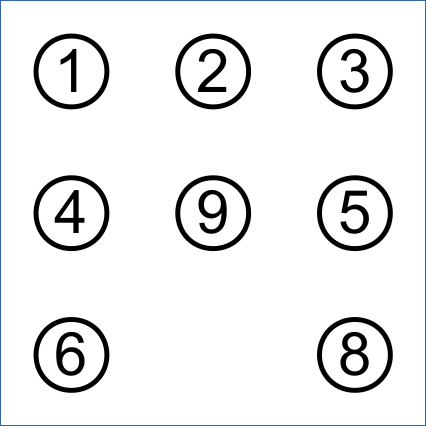
\includegraphics[scale=1]{../folien/symbol.png}
\caption[Bestückungspositionen]{Bestückungspositionen von TOP aus gesehen}
\end{figure}

Zentrales Bauteil der Hardware ist der Microcontroller \href{https://www.microchip.com/wwwproducts/en/ATtiny804}{ATtiny804} der Firma Microchip. Er übersetzt die Statusbefehle vom Stellwerksrechner in die entsprechende Ansteuerung der LEDs bzw. meldet eine Änderung des Tastenzustandes.

Die Kommunikation mit dem Stellwerksrechner wird über einen 5V I\textsuperscript{2}C Bus mit $100k\frac{bit}{s}$ Übertragungsrate hergestellt. 

Die Gleissymbole nehmen an der Kommunikation als Slave teil. Nur bei einer Änderung des Tastenzustandes übernimmt das Gleisfeld die Buskontrolle.
\subsection{Steckerbelegung}
Die einzelnen Module werden mittels Flachbandkabel untereinander verbunden. Jede Steckerposition am Kabel ist gleich.
\begin{table}[h!]
\centering
\begin{tabular}{c|l|l}
\textbf{Pin} & \textbf{Name} & \textbf{Beschreibung}\\ \hline
\multirow{2} {*}{1} & \multirow{2} {*}{BLINK} & Phasensignal wenn die LEDs blinken.\\
& & Blink=0 entspricht LED leuchtet.\\ 
2 & SCL & I\textsuperscript{2}C Takt\\ 
3 & GND & Masse \\ 
4 & SDA & I\textsuperscript{2}C Daten\\ 
\multirow{2}{*}{5} & \multirow{2}{*}{UPDI} & Debug und Programmierleitung.\\
& & Wird im Normalbetrieb nicht verwendet.\\
6 & VCC & Versorgungsspannung (5V)
\end{tabular}
\caption{Steckerbelegung}
\end{table}
\begin{figure}[hbtp!]
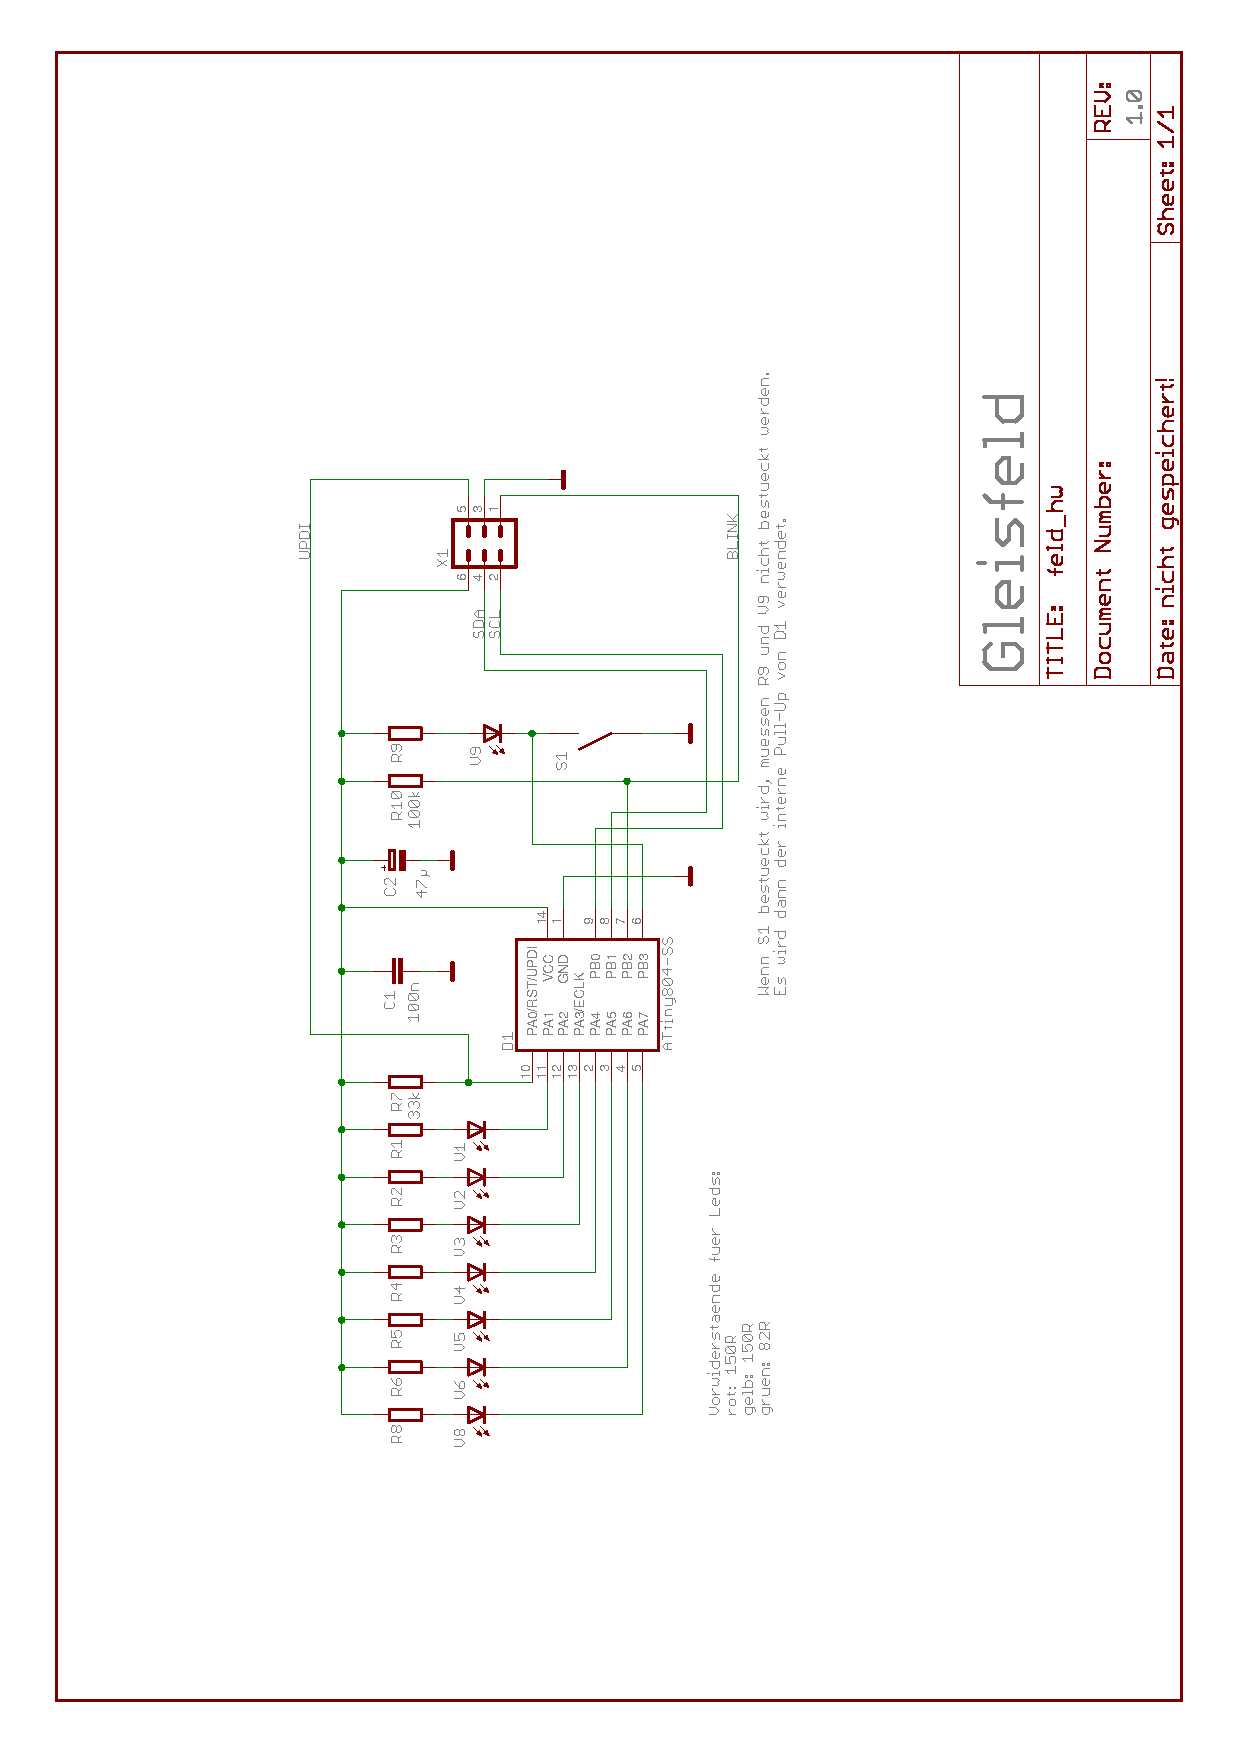
\includegraphics[scale=0.7]{feld_hw.pdf}
\caption{Schaltplan}
\end{figure}
\begin{figure}[hbtp!]
\centering
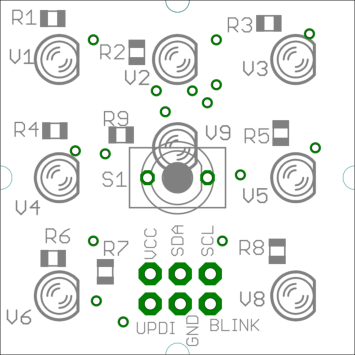
\includegraphics[width=6cm]{feld_hw_top_comp.pdf}
\caption[Bestückungsplan TOP]{Bestückungsplan TOP (Masstab 2:1)}
\end{figure}
\begin{figure}[hbtp!]
\centering
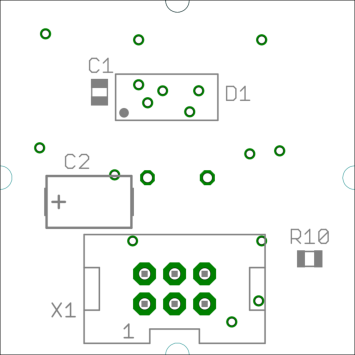
\includegraphics[width=6cm]{feld_hw_bot_comp.pdf}
\caption[Bestückungsplan BOT]{Bestückungsplan BOT (Masstab 2:1)}
\end{figure}
\newpage
\section{Symboltypen}


\subsection{Gleis Gerade (G1)}
\begin{figure}[hbtp]
\centering
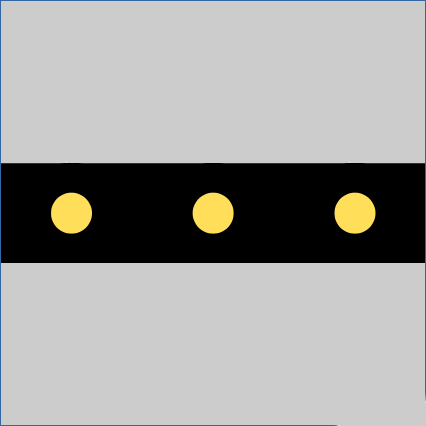
\includegraphics[width=3cm]{../folien/g1.png}
\caption{Symbol G1}
\end{figure}
\begin{table}[h!]
\centering
\begin{tabular}{c|c}
\textbf{Pos} & \textbf{Funktion} \\ \hline
4 & LED gelb \\
5 & LED gelb \\
9 & LED gelb
\end{tabular}
\caption{Bestückung G1}
\end{table}
\begin{table}[h!]
\centering
\begin{tabular}{c|c}
\textbf{Zustand} & \textbf{Beschreibung} \\ \hline
FREE & alle LEDs sind aus \\
PATH\_PENDING & alle LEDs blinken \\
PATH\_LOCKED & alle LEDs sind ein
\end{tabular}
\caption{Zustände G1}
\end{table}

\newpage
\subsection{Gleis Diagonale (D1)}
\begin{figure}[hbtp]
\centering

\includegraphics[width=3cm]{../folien/d1.png}
\caption{Symbol D1}
\end{figure}
\begin{table}[h!]
\centering
\begin{tabular}{c|c}
\textbf{Pos} & \textbf{Funktion} \\ \hline
3 & LED gelb \\
6 & LED gelb \\
9 & LED gelb
\end{tabular}
\caption{Bestückung D1}
\end{table}
\begin{table}[h!]
\centering
\begin{tabular}{c|c}
\textbf{Zustand} & \textbf{Beschreibung} \\ \hline
FREE & alle LEDs sind aus \\
PATH\_PENDING & alle LEDs blinken \\
PATH\_LOCKED & alle LEDs sind ein
\end{tabular}
\caption{Zustände D1}
\end{table}

\newpage
\subsection{Gleis Bogen rechts (B1)}
\begin{figure}[hbtp]
\centering

\includegraphics[width=3cm]{../folien/b1.png}
\caption{Symbol B1}
\end{figure}
\begin{table}[h!]
\centering
\begin{tabular}{c|c}
\textbf{Pos} & \textbf{Funktion} \\ \hline
1 & LED gelb \\
5 & LED gelb \\
9 & LED gelb
\end{tabular}
\caption{Bestückung B1}
\end{table}
\begin{table}[h!]
\centering
\begin{tabular}{c|c}
\textbf{Zustand} & \textbf{Beschreibung} \\ \hline
FREE & alle LEDs sind aus \\
PATH\_PENDING & alle LEDs blinken \\
PATH\_LOCKED & alle LEDs sind ein
\end{tabular}
\caption{Zustände B1}
\end{table}


\newpage
\subsection{Gleis Bogen links (B2)}
\begin{figure}[hbtp]
\centering

\includegraphics[width=3cm]{../folien/b2.png}
\caption{Symbol B2}
\end{figure}
\begin{table}[h!]
\centering
\begin{tabular}{c|c}
\textbf{Pos} & \textbf{Funktion} \\ \hline
3 & LED gelb \\
4 & LED gelb \\
9 & LED gelb
\end{tabular}
\caption{Bestückung B2}
\end{table}
\begin{table}[h!]
\centering
\begin{tabular}{c|c}
\textbf{Zustand} & \textbf{Beschreibung} \\ \hline
FREE & alle LEDs sind aus \\
PATH\_PENDING & alle LEDs blinken \\
PATH\_LOCKED & alle LEDs sind ein
\end{tabular}
\caption{Zustände B2}
\end{table}

\newpage
\subsection{Gleis Funktion gerade (F1)}
Entspricht einer allgemeinen Funktionstaste. Mögliche Funktionen sind z.B. Entkuppler oder Fahrstraßenanfangs oder -endtaste.
\begin{figure}[hbtp]
\centering
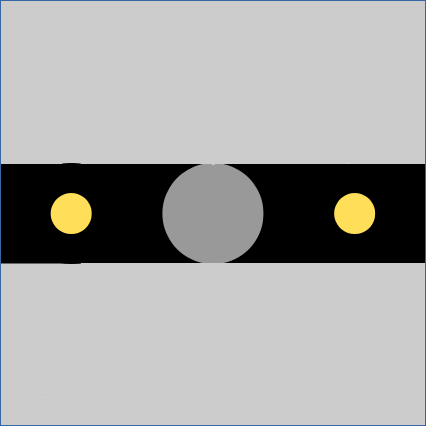
\includegraphics[width=3cm]{../folien/f1.png}
\caption{Symbol F1}
\end{figure}
\begin{table}[h!]
\centering
\begin{tabular}{c|c}
\textbf{Pos} & \textbf{Funktion} \\ \hline
4 & LED gelb \\
5 & LED gelb \\
9 & Taster
\end{tabular}
\caption{Bestückung F1}
\end{table}
\begin{table}[h!]
\centering
\begin{tabular}{c|c}
\textbf{Zustand} & \textbf{Beschreibung} \\ \hline
FREE & alle LEDs sind aus \\
PATH\_PENDING & alle LEDs blinken \\
PATH\_LOCKED & alle LEDs sind ein \\
QUIET & Tastenevents dürfen nicht gemeldet werden
\end{tabular}
\caption{Zustände F1}
\end{table}

\newpage
\subsection{Gleis Funktion diagonale (F2)}
Entspricht einer allgemeinen Funktionstaste. Mögliche Funktionen sind z.B. Entkuppler oder Fahrstraßenanfangs oder -endtaste.
\begin{figure}[hbtp]
\centering
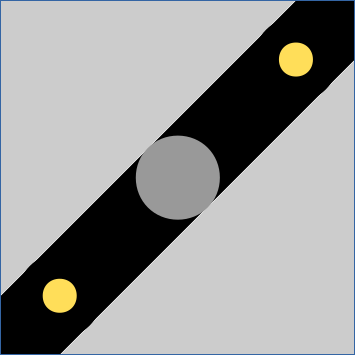
\includegraphics[width=3cm]{../folien/f2.png}
\caption{Symbol F2}
\end{figure}
\begin{table}[h!]
\centering
\begin{tabular}{c|c}
\textbf{Pos} & \textbf{Funktion} \\ \hline
3 & LED gelb \\
6 & LED gelb \\
9 & Taster
\end{tabular}
\caption{Bestückung F2}
\end{table}
\begin{table}[h!]
\centering
\begin{tabular}{c|c}
\textbf{Zustand} & \textbf{Beschreibung} \\ \hline
FREE & alle LEDs sind aus \\
PATH\_PENDING & alle LEDs blinken \\
PATH\_LOCKED & alle LEDs sind ein \\
QUIET & Tastenevents dürfen nicht gemeldet werden
\end{tabular}
\caption{Zustände F2}
\end{table}

\newpage
\subsection{Gleis Funktion Boggen rechts (F3)}
Entspricht einer allgemeinen Funktionstaste. Mögliche Funktionen sind z.B. Entkuppler oder Fahrstraßenanfangs oder -endtaste.
\begin{figure}[hbtp]
\centering
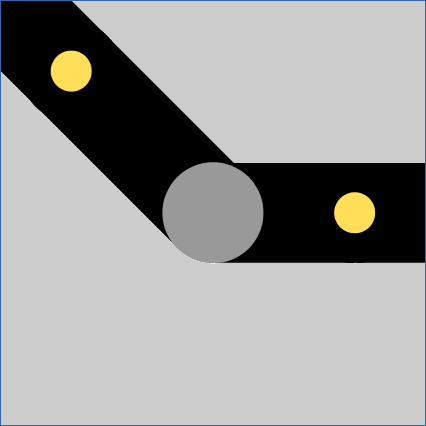
\includegraphics[width=3cm]{../folien/f3.png}
\caption{Symbol F3}
\end{figure}
\begin{table}[h!]
\centering
\begin{tabular}{c|c}
\textbf{Pos} & \textbf{Funktion} \\ \hline
3 & LED gelb \\
6 & LED gelb \\
9 & Taster
\end{tabular}
\caption{Bestückung F3}
\end{table}
\begin{table}[h!]
\centering
\begin{tabular}{c|c}
\textbf{Zustand} & \textbf{Beschreibung} \\ \hline
FREE & alle LEDs sind aus \\
PATH\_PENDING & alle LEDs blinken \\
PATH\_LOCKED & alle LEDs sind ein \\
QUIET & Tastenevents dürfen nicht gemeldet werden
\end{tabular}
\caption{Zustände F3}
\end{table}
 
 \newpage
\subsection{Gleis Funktion Bogen links (F4)}
Entspricht einer allgemeinen Funktionstaste. Mögliche Funktionen sind z.B. Entkuppler oder Fahrstraßenanfangs oder -endtaste.
\begin{figure}[hbtp]
\centering
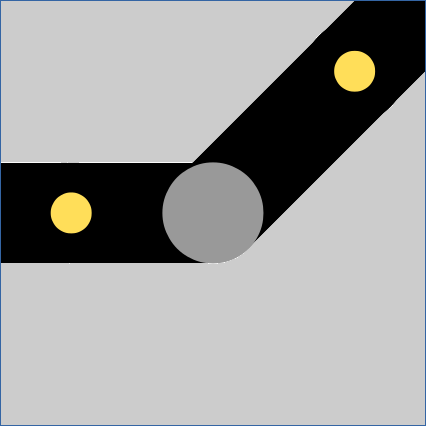
\includegraphics[width=3cm]{../folien/f4.png}
\caption{Symbol F4}
\end{figure}
\begin{table}[h!]
\centering
\begin{tabular}{c|c}
\textbf{Pos} & \textbf{Funktion} \\ \hline
3 & LED gelb \\
6 & LED gelb \\
9 & Taster
\end{tabular}
\caption{Bestückung F4}
\end{table}
\begin{table}[h!]
\centering
\begin{tabular}{c|c}
\textbf{Zustand} & \textbf{Beschreibung} \\ \hline
FREE & alle LEDs sind aus \\
PATH\_PENDING & alle LEDs blinken \\
PATH\_LOCKED & alle LEDs sind ein \\
QUIET & Tastenevents dürfen nicht gemeldet werden
\end{tabular}
\caption{Zustände F4}
\end{table}

\newpage
\subsection{Gleis Weiche rechts (W1)}
Einfache Weiche rechts.
\begin{figure}[hbtp]
\centering
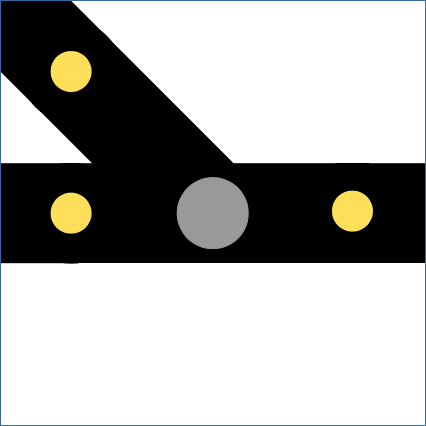
\includegraphics[width=3cm]{../folien/w1.png}
\caption{Symbol W1}
\end{figure}
\begin{table}[h!]
\centering
\begin{tabular}{c|c}
\textbf{Pos} & \textbf{Funktion} \\ \hline
1 & LED gelb \\
4 & LED gelb \\
5 & LED gelb \\
9 & Taster
\end{tabular}
\caption{Bestückung W1}
\end{table}
\begin{table}[h!]
\centering
\begin{tabular}{c|c}
\textbf{Zustand} & \textbf{Beschreibung} \\ \hline
FREE & alle LEDs sind aus \\
PATH\_PENDING & aktive LEDs blinken \\
PATH\_LOCKED & aktive LEDs sind ein \\
STRAIT & Positionen 4 und 5 sind aktiv \\
TURN & Positionen 1 und 5 sind aktiv\\
QUIET & Tastenevents dürfen nicht gemeldet werden
\end{tabular}
\caption{Zustände W1}
\end{table}

 \newpage
\subsection{Gleis Weiche links (W2)}
Einfache Weiche rechts.
\begin{figure}[hbtp]
\centering
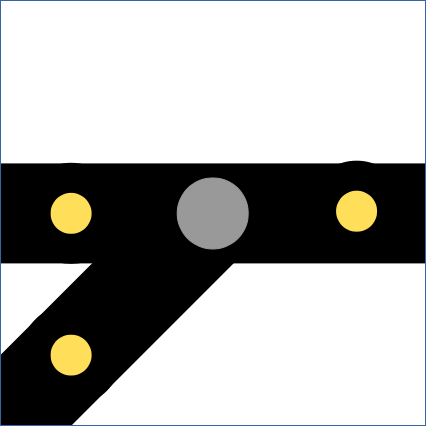
\includegraphics[width=3cm]{../folien/w2.png}
\caption{Symbol W2}
\end{figure}
\begin{table}[h!]
\centering
\begin{tabular}{c|c}
\textbf{Pos} & \textbf{Funktion} \\ \hline
4 & LED gelb \\
5 & LED gelb \\
6 & LED gelb \\
9 & Taster
\end{tabular}
\caption{Bestückung W2}
\end{table}
\begin{table}[h!]
\centering
\begin{tabular}{c|c}
\textbf{Zustand} & \textbf{Beschreibung} \\ \hline
FREE & alle LEDs sind aus \\
PATH\_PENDING & aktive LEDs blinken \\
PATH\_LOCKED & aktive LEDs sind ein \\
STRAIT & Positionen 4 und 5 sind aktiv \\
TURN & Positionen 5 und 6 sind aktiv\\
QUIET & Tastenevents dürfen nicht gemeldet werden
\end{tabular}
\caption{Zustände W2}
\end{table}

\newpage
\subsection{Gleis Weiche rechts diagonal (W3)}
Einfache Weiche rechts.
\begin{figure}[hbtp]
\centering
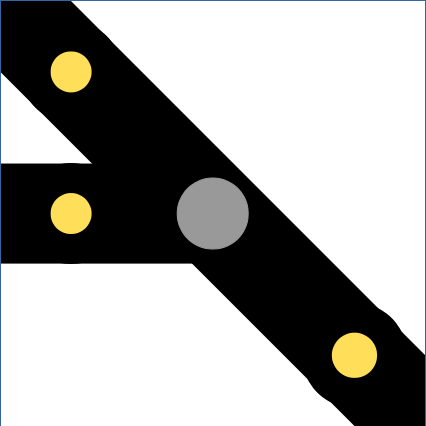
\includegraphics[width=3cm]{../folien/w3.png}
\caption{Symbol W3}
\end{figure}
\begin{table}[h!]
\centering
\begin{tabular}{c|c}
\textbf{Pos} & \textbf{Funktion} \\ \hline
3 & LED gelb \\
5 & LED gelb \\
6 & LED gelb \\
9 & Taster
\end{tabular}
\caption{Bestückung W3}
\end{table}
\begin{table}[h!]
\centering
\begin{tabular}{c|c}
\textbf{Zustand} & \textbf{Beschreibung} \\ \hline
FREE & alle LEDs sind aus \\
PATH\_PENDING & aktive LEDs blinken \\
PATH\_LOCKED & aktive LEDs sind ein \\
STRAIT & Positionen 3 und 6 sind aktiv \\
TURN & Positionen 5 und 6 sind aktiv\\
QUIET & Tastenevents dürfen nicht gemeldet werden
\end{tabular}
\caption{Zustände W3}
\end{table}

\newpage
\subsection{Gleis Weiche links diagonal (W4)}
Einfache Weiche rechts.
\begin{figure}[hbtp]
\centering
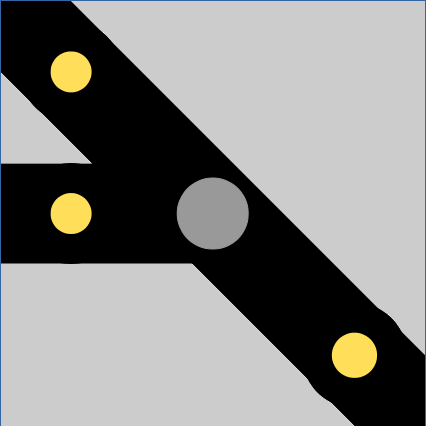
\includegraphics[width=3cm]{../folien/w4.png}
\caption{Symbol W4}
\end{figure}
\begin{table}[h!]
\centering
\begin{tabular}{c|c}
\textbf{Pos} & \textbf{Funktion} \\ \hline
1 & LED gelb \\
4 & LED gelb \\
8 & LED gelb \\
9 & Taster
\end{tabular}
\caption{Bestückung W4}
\end{table}
\begin{table}[h!]
\centering
\begin{tabular}{c|c}
\textbf{Zustand} & \textbf{Beschreibung} \\ \hline
FREE & alle LEDs sind aus \\
PATH\_PENDING & aktive LEDs blinken \\
PATH\_LOCKED & aktive LEDs sind ein \\
STRAIT & Positionen 1 und 8 sind aktiv \\
TURN & Positionen 4 und 8 sind aktiv\\
QUIET & Tastenevents dürfen nicht gemeldet werden
\end{tabular}
\caption{Zustände W4}
\end{table}

\end{document}